\chapter{Aufgabe 3}

\noindent
Die in den Lösungsvorschlägen angegebene Reihenfolge dient nur zur Veranschaulichung und entspricht nicht notwendigerweise der in den Spezifikationen hinterlegten Reihenfolge.

\section{Teil a)}
IPSec im \textbf{Transportmodus} (s. Abbildung~\ref{fig:transportmodus}):

\begin{enumerate}
    \itemsep0.5em
    \item Der original IP-Header wird im \textbf{Transportmodus} beibehalten
    \item Erzeugung des IPSec-Headers, der je nach verwendetem IPSec-Protokoll aufgebaut ist (\textit{Authentication Header AH}~\cite{RFC4302} oder \textit{Encapsulating Security Payload ESP}~\cite{RFC4303}) - bei \textit{AH} wird hierzu insbesondere noch der \textit{HMAC} generiert (unter Berücksichtigung der Nutzdaten, des AH-Headers und Feldern des IP-Headers, die nicht geändert werden\footnote{
    bestimmte Felder eines IP-Headers unterliegen Änderungen, während sie von Knotenpunkt zu Knotenpunkt geleitet werden, wie bspw. das IPv4 \textit{TTL}-Feld (\textit{Time-To-Live},~\cite[360 ff.]{KR14}), und dürfen deshalb nicht zur Generierung des HMAC miteinbezogen werden.
    })

    \item Einbettung des IPSec-Headers nach dem originalen IP-Header
    \item Einbettung der Payloads nach dem IPSec-Header; im Fall von ESP: \textbf{verschlüsselt}
    \item Falls \textit{ESP} verwendet wird: Erzeugung und Anhängen des ESP-Trailers
\end{enumerate}

\begin{figure}
    \centering
    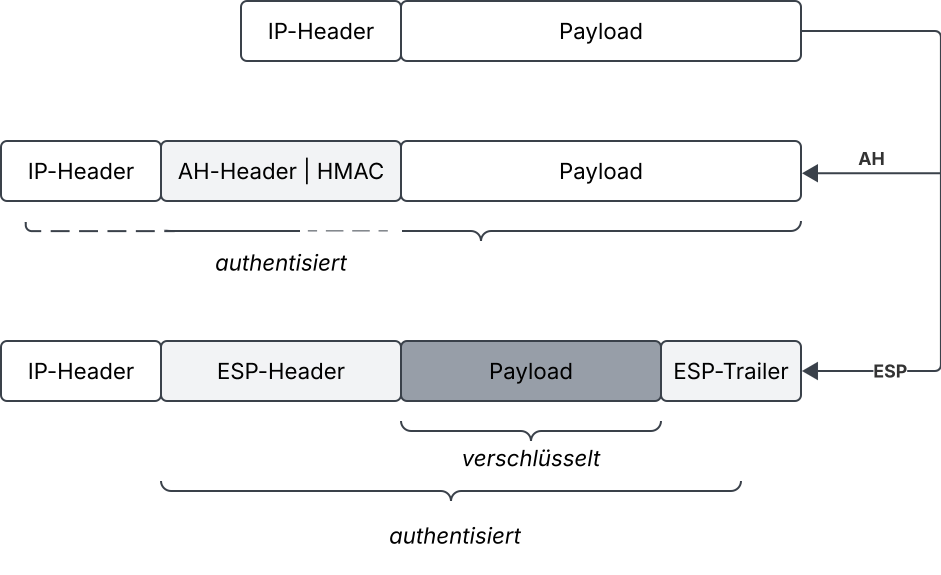
\includegraphics[scale=0.4]{aufgabe 3/img/transportmodus.svg}
    \caption{Skizze von IPSec im Transportmodus unter Anwendung von \textit{AH} bzw. \textit{ESP}. \textit{AH} sorgt insbesondere für Authentizität und Integrität, während ESP durch die Verschlüsselung zusätzlich Vertraulichkeit garantiert. Hervorzuheben ist an dieser Stelle, dass bei AH Teile des IP-Headers für Authentisierung miteinbezogen werden, weshalb man die Protokolle auch in Kombination einsetzt. (Quelle: In Anlehnung an~\cite[\textbf{Abb. 3.6}, 41]{ITS4})}
    \label{fig:transportmodus}
\end{figure}

\section{Teil b)}
IPSec im \textbf{Tunnelmodus} (s. Abbildung~\ref{fig:tunnelmodus}):

\begin{enumerate}
    \itemsep0.5em
    \item Erzeugung eines neuen IP-Headers mit den Adressinformationen, insb. Zieladresse IPSec-Gateway
    \item Erzeugung des IPSec Headers (unter gleichen Bedingungen wie in Lösungsvorschlag zu Aufgabenteil a) angegeben)
    \item Einbettung des IPSec-Headers nach dem \textbf{neuen} IP-Header
    \item Einbettung des originalen IP-Headers und Payloads nach dem IPSec-Header (im Fall von ESP: Verschlüsselung der original IP-Headers und Payload)
    \item Falls \textit{ESP} verwendet wird: Erzeugung und Anhängen des ESP-Trailers
\end{enumerate}

\begin{figure}
    \centering
    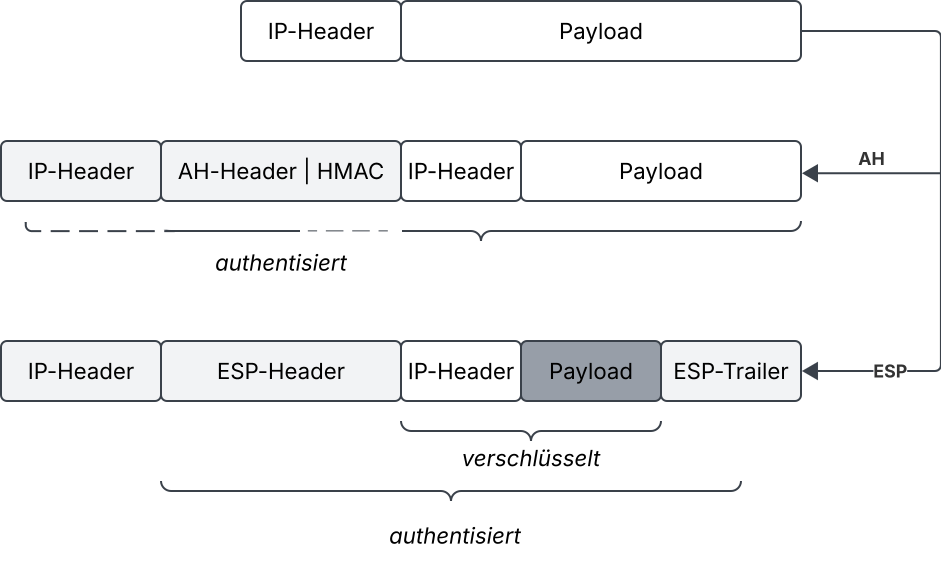
\includegraphics[scale=0.4]{aufgabe 3/img/tunnelmodus.svg}
    \caption{Skizze von IPSec im Tunnelmodus unter Anwendung von \textit{AH} bzw. \textit{ESP}. (Quelle: In Anlehnung an~\cite[\textbf{Abb. 3.6}, 41]{ITS4})}
    \label{fig:tunnelmodus}
\end{figure}